\documentclass[11pt]{amsart}

\usepackage{amsmath}
\usepackage{physics}
\usepackage{graphicx}

\renewcommand{\thesubsection}{\thesection.\alph{subsection}}

\title[Vibrations and Phonons]{Vibrations and Phonons \\
		\hrulefill \small{ FYS3410: Problem Sheet 2 } \hrulefill}
	
\author{Candidate 33}


\begin{document}

\maketitle

\section{Vibrations of a One-Dimensional Monatomic Chain}
This is a study of the vibrations in an infinite one-dimensional crystal with just one atom in  the basis. 

\subsection{Dispersion Relation}
If the temperature of the  crystal is low enough one can model the crystal as a chain of masses held together by springs with length $a$, which is also the lattice constant. Hooke's law can be used to model the force between the atoms,
\begin{equation}
F = g\delta x,
\end{equation}
where $g$ is the spring constant and $\delta x$ is the displacement of a particular mass. Such a model is often referred to as a \emph{harmonic} chain.

The position of atom $n$ in the lattice is $x_n$. The equilibrium position of this atom is $x_n^{eq} = na$. Once we allow for motion of the atoms $x_n$ will deviate from the equilibrium position,
\begin{equation}
\delta x_n = x_n - x_n^{eq}.
\end{equation}
The force acting on mass $n$ in the chain is then given by
\begin{equation}
F_n = g(\delta x_{n+1} - \delta x_n) + g(\delta x_{n-1} - \delta x_n),
\end{equation}
when taking into consideration the atoms of each side of atom $n$. Thus we have Newton's equation of motion
\begin{equation}
\label{eq:N2L}
m(\delta \ddot{x}_n) = F_n = g(\delta x_{n+1} + g(\delta x_{n-1} - 2\delta x_n).
\end{equation}
A good guess to a solution to this equation is
\begin{equation}
\label{eq:oscillatorsolution}
\delta x_n = Ae^{i\omega t - ikx_n^{eq}}=Ae^{i\omega t - ikna},
\end{equation}
where $A$ is the amplitude of the oscillation, and $k$ and $\omega$ are the wavevector and frequency of the proposed wave. The only thing a bit strange here is that there are, apparently, complex values of $\delta x_n$. The complex numbers are used for convenience, but actually the real part of the expression is implied.

Inserting equation \ref{eq:oscillatorsolution} into equation \ref{eq:N2L} yields
\begin{align*}
-m\omega^2Ae^{ik\omega t - ikna} &= gAe^{i\omega t}(e^{-ikna(n+1)} + e^{-ika(n-1)} - 2e^{-ikan}), \\
m\omega^2 &= 2g(1-\cos ka) = 4g\sin^2 \frac{ka}{2}.
\end{align*}
From this the desired result is obtained
\begin{equation}
\omega = 2\sqrt{\frac{g}{m}}\abs{\sin{\frac{ka}{2}}},
\end{equation}
which is a general relationship between a frequency (energy) and a wavevector (momentum) known as a \emph{dispersion relation}.

\subsection{Visualisation of the Dispersion Relation}
One can see from the plot in figure \ref{fig:brillouin_dispersion} how the dispersion relation repeats after the first Brillouin zone, indicated by dashed lines. The dispersion is in fact periodic in $k \rightarrow k + 2\pi/a$. When one knows the dispersion relation for the first Brillouin zone, one knows the dispersion relation everywhere.

\begin{figure}
\centering
	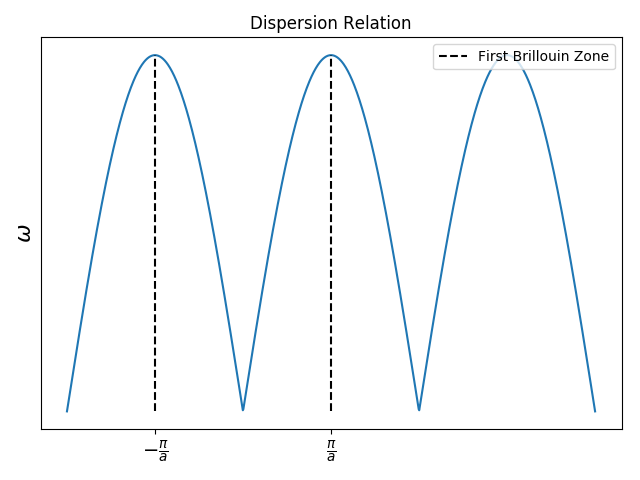
\includegraphics[width=0.7\textwidth]{first_brillouin.png}
	\caption{The dispersion relation is repeated after the first Brillouin zone.}
	\label{fig:brillouin_dispersion}
\end{figure}

\subsection{Group Velocity}
The group velocity is given by
\begin{equation}
v_g = \frac{\Delta \omega}{\Delta k},
\end{equation}
for an infinitesimal change this is equal to the derivative of the dispersion relation with regards to $k$. By looking at the graph in figure \ref{fig:brillouin_dispersion}, one can see that the group velocity must be highest at the center of the first Brillouin zone. The group velocity is decreasing towards zero as one gets closer to the edge of the first Brillouin zone. 

\subsection{Maximum Amplitude of Na-crystal}
Imagine a longitudinal wave propagating in direction [100], given by Miller indices, in a sodium (Na) crystal.

Limiting the viewpoint again to the  first Brillouin zone ($k\pm+pi/a$) gives a standing wave defined by 
\begin{equation}
\delta_n = Ae^{i\omega t - ikna}
\end{equation}

\end{document}